% !TEX root = ../../../main.tex
% 来源：高中物理甲种本·第三册（电磁·光学·近代物理）
% 章节：光的反射和折射 / 折射率
% 原始文件：5.tex，行 780-798
% 类型：tikz
% ---
	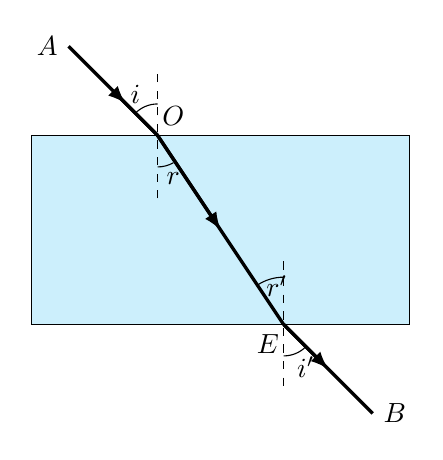
\begin{tikzpicture}[>=latex, scale=.8]
\draw [fill=cyan!20] (-3,-3) rectangle (3,0);
\draw [very thick](-1,0)--(1,-3);	
\node at (-.75,0)[above]{$O$};
\node at (.75,-3)[below]{$E$};
\draw[->, very thick](-1,0)--(0,-1.5)	;
\draw[very thick] (-1,0)--+(135:2)node [left]{$A$};
\draw[very thick] (1,-3)--+(-45:2)node [right]{$B$};
\draw[very thick, -<] (-1,0)--+(135:1);
\draw[very thick, ->] (1,-3)--+(-45:1);
	\draw[dashed] (-1,-1)--(-1,1);
	\draw[dashed] (1,-2)--(1,-4);
\draw (-1,0.5) arc (90:135:.5)node[above]{$i$};
\draw (1,-3.5) arc (-90:-45:.5)node[below]{$i'$};
\draw (-1,-0.5) arc (-90:-60:.5)node[below]{$r$};
\draw (1,-2.25) arc (90:125:.75)node[right]{$r'$};


	\end{tikzpicture}
